% Created by tikzDevice version 0.12.6 on 2024-03-24 19:10:44
% !TEX encoding = UTF-8 Unicode
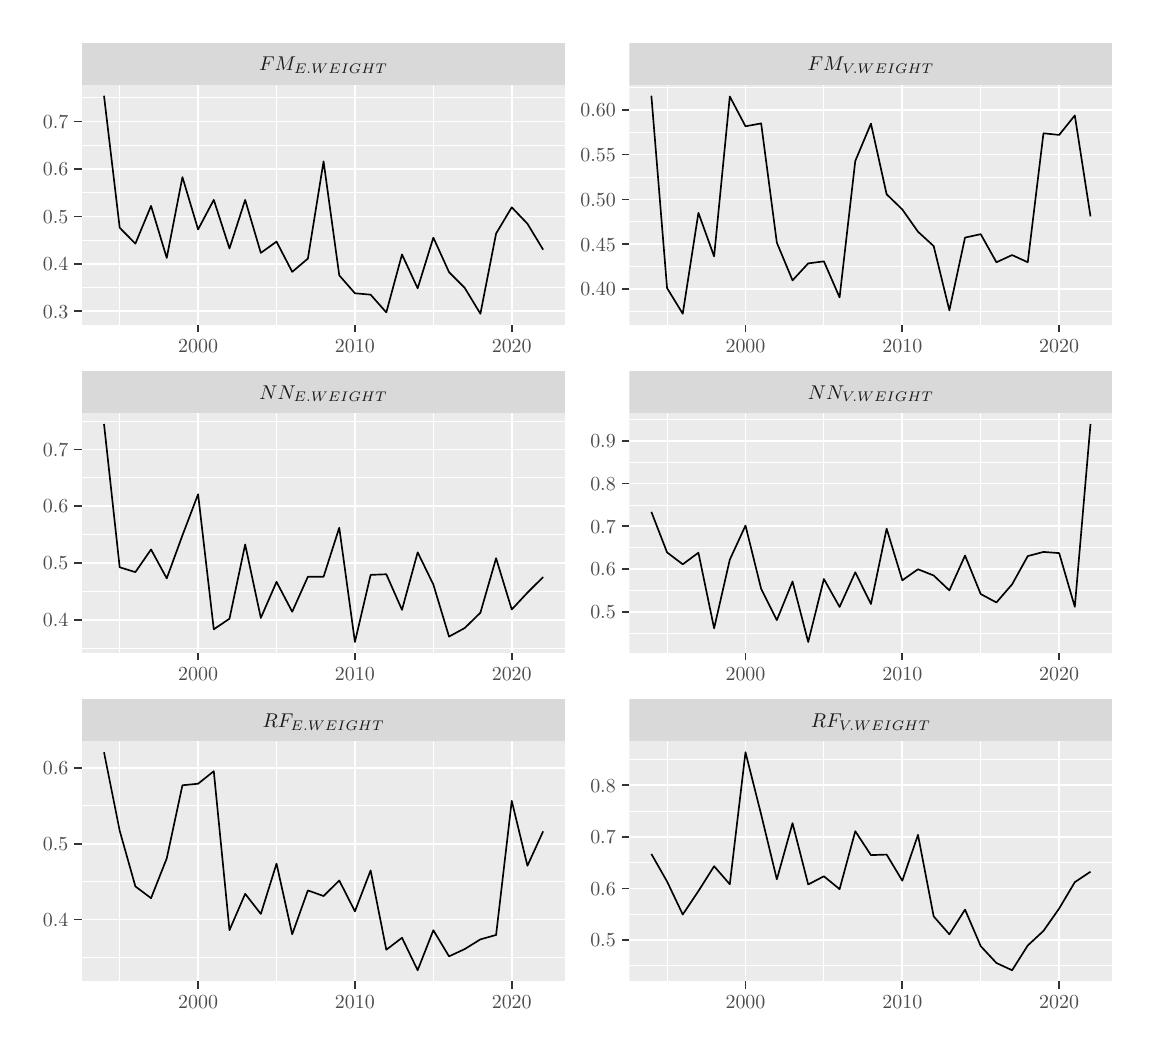
\begin{tikzpicture}[x=1pt,y=1pt]
\definecolor{fillColor}{RGB}{255,255,255}
\path[use as bounding box,fill=fillColor,fill opacity=0.00] (0,0) rectangle (397.48,361.35);
\begin{scope}
\path[clip] (  0.00,  0.00) rectangle (397.48,361.35);
\definecolor{drawColor}{RGB}{255,255,255}
\definecolor{fillColor}{RGB}{255,255,255}

\path[draw=drawColor,line width= 0.6pt,line join=round,line cap=round,fill=fillColor] (  0.00,  0.00) rectangle (397.48,361.35);
\end{scope}
\begin{scope}
\path[clip] ( 19.65,254.04) rectangle (194.19,340.69);
\definecolor{fillColor}{gray}{0.92}

\path[fill=fillColor] ( 19.65,254.04) rectangle (194.19,340.69);
\definecolor{drawColor}{RGB}{255,255,255}

\path[draw=drawColor,line width= 0.3pt,line join=round] ( 19.65,267.42) --
	(194.19,267.42);

\path[draw=drawColor,line width= 0.3pt,line join=round] ( 19.65,284.57) --
	(194.19,284.57);

\path[draw=drawColor,line width= 0.3pt,line join=round] ( 19.65,301.72) --
	(194.19,301.72);

\path[draw=drawColor,line width= 0.3pt,line join=round] ( 19.65,318.87) --
	(194.19,318.87);

\path[draw=drawColor,line width= 0.3pt,line join=round] ( 19.65,336.02) --
	(194.19,336.02);

\path[draw=drawColor,line width= 0.3pt,line join=round] ( 33.25,254.04) --
	( 33.25,340.69);

\path[draw=drawColor,line width= 0.3pt,line join=round] ( 89.92,254.04) --
	( 89.92,340.69);

\path[draw=drawColor,line width= 0.3pt,line join=round] (146.59,254.04) --
	(146.59,340.69);

\path[draw=drawColor,line width= 0.6pt,line join=round] ( 19.65,258.85) --
	(194.19,258.85);

\path[draw=drawColor,line width= 0.6pt,line join=round] ( 19.65,276.00) --
	(194.19,276.00);

\path[draw=drawColor,line width= 0.6pt,line join=round] ( 19.65,293.15) --
	(194.19,293.15);

\path[draw=drawColor,line width= 0.6pt,line join=round] ( 19.65,310.30) --
	(194.19,310.30);

\path[draw=drawColor,line width= 0.6pt,line join=round] ( 19.65,327.45) --
	(194.19,327.45);

\path[draw=drawColor,line width= 0.6pt,line join=round] ( 61.58,254.04) --
	( 61.58,340.69);

\path[draw=drawColor,line width= 0.6pt,line join=round] (118.25,254.04) --
	(118.25,340.69);

\path[draw=drawColor,line width= 0.6pt,line join=round] (174.92,254.04) --
	(174.92,340.69);
\definecolor{drawColor}{RGB}{0,0,0}

\path[draw=drawColor,line width= 0.6pt,line join=round] ( 27.58,336.75) --
	( 33.25,289.05) --
	( 38.92,283.31) --
	( 44.58,296.95) --
	( 50.25,278.14) --
	( 55.92,307.35) --
	( 61.58,288.44) --
	( 67.25,299.14) --
	( 72.92,281.57) --
	( 78.59,299.11) --
	( 84.25,279.97) --
	( 89.92,284.03) --
	( 95.59,273.11) --
	(101.25,277.90) --
	(106.92,313.03) --
	(112.59,271.85) --
	(118.25,265.37) --
	(123.92,264.87) --
	(129.59,258.45) --
	(135.26,279.40) --
	(140.92,267.16) --
	(146.59,285.49) --
	(152.26,273.01) --
	(157.92,267.33) --
	(163.59,257.98) --
	(169.26,286.96) --
	(174.92,296.43) --
	(180.59,290.50) --
	(186.26,281.13);
\end{scope}
\begin{scope}
\path[clip] ( 19.65,135.43) rectangle (194.19,222.07);
\definecolor{fillColor}{gray}{0.92}

\path[fill=fillColor] ( 19.65,135.43) rectangle (194.19,222.07);
\definecolor{drawColor}{RGB}{255,255,255}

\path[draw=drawColor,line width= 0.3pt,line join=round] ( 19.65,137.17) --
	(194.19,137.17);

\path[draw=drawColor,line width= 0.3pt,line join=round] ( 19.65,157.68) --
	(194.19,157.68);

\path[draw=drawColor,line width= 0.3pt,line join=round] ( 19.65,178.20) --
	(194.19,178.20);

\path[draw=drawColor,line width= 0.3pt,line join=round] ( 19.65,198.71) --
	(194.19,198.71);

\path[draw=drawColor,line width= 0.3pt,line join=round] ( 19.65,219.23) --
	(194.19,219.23);

\path[draw=drawColor,line width= 0.3pt,line join=round] ( 33.25,135.43) --
	( 33.25,222.07);

\path[draw=drawColor,line width= 0.3pt,line join=round] ( 89.92,135.43) --
	( 89.92,222.07);

\path[draw=drawColor,line width= 0.3pt,line join=round] (146.59,135.43) --
	(146.59,222.07);

\path[draw=drawColor,line width= 0.6pt,line join=round] ( 19.65,147.42) --
	(194.19,147.42);

\path[draw=drawColor,line width= 0.6pt,line join=round] ( 19.65,167.94) --
	(194.19,167.94);

\path[draw=drawColor,line width= 0.6pt,line join=round] ( 19.65,188.46) --
	(194.19,188.46);

\path[draw=drawColor,line width= 0.6pt,line join=round] ( 19.65,208.97) --
	(194.19,208.97);

\path[draw=drawColor,line width= 0.6pt,line join=round] ( 61.58,135.43) --
	( 61.58,222.07);

\path[draw=drawColor,line width= 0.6pt,line join=round] (118.25,135.43) --
	(118.25,222.07);

\path[draw=drawColor,line width= 0.6pt,line join=round] (174.92,135.43) --
	(174.92,222.07);
\definecolor{drawColor}{RGB}{0,0,0}

\path[draw=drawColor,line width= 0.6pt,line join=round] ( 27.58,218.14) --
	( 33.25,166.36) --
	( 38.92,164.61) --
	( 44.58,172.80) --
	( 50.25,162.35) --
	( 55.92,177.89) --
	( 61.58,192.76) --
	( 67.25,143.94) --
	( 72.92,147.78) --
	( 78.59,174.59) --
	( 84.25,148.06) --
	( 89.92,161.09) --
	( 95.59,150.29) --
	(101.25,162.94) --
	(106.92,162.93) --
	(112.59,180.66) --
	(118.25,139.36) --
	(123.92,163.61) --
	(129.59,163.84) --
	(135.26,150.98) --
	(140.92,171.76) --
	(146.59,160.12) --
	(152.26,141.32) --
	(157.92,144.40) --
	(163.59,149.94) --
	(169.26,169.62) --
	(174.92,151.11) --
	(180.59,157.19) --
	(186.26,162.82);
\end{scope}
\begin{scope}
\path[clip] ( 19.65, 16.81) rectangle (194.19,103.46);
\definecolor{fillColor}{gray}{0.92}

\path[fill=fillColor] ( 19.65, 16.81) rectangle (194.19,103.46);
\definecolor{drawColor}{RGB}{255,255,255}

\path[draw=drawColor,line width= 0.3pt,line join=round] ( 19.65, 25.40) --
	(194.19, 25.40);

\path[draw=drawColor,line width= 0.3pt,line join=round] ( 19.65, 52.78) --
	(194.19, 52.78);

\path[draw=drawColor,line width= 0.3pt,line join=round] ( 19.65, 80.16) --
	(194.19, 80.16);

\path[draw=drawColor,line width= 0.3pt,line join=round] ( 33.25, 16.81) --
	( 33.25,103.46);

\path[draw=drawColor,line width= 0.3pt,line join=round] ( 89.92, 16.81) --
	( 89.92,103.46);

\path[draw=drawColor,line width= 0.3pt,line join=round] (146.59, 16.81) --
	(146.59,103.46);

\path[draw=drawColor,line width= 0.6pt,line join=round] ( 19.65, 39.09) --
	(194.19, 39.09);

\path[draw=drawColor,line width= 0.6pt,line join=round] ( 19.65, 66.47) --
	(194.19, 66.47);

\path[draw=drawColor,line width= 0.6pt,line join=round] ( 19.65, 93.85) --
	(194.19, 93.85);

\path[draw=drawColor,line width= 0.6pt,line join=round] ( 61.58, 16.81) --
	( 61.58,103.46);

\path[draw=drawColor,line width= 0.6pt,line join=round] (118.25, 16.81) --
	(118.25,103.46);

\path[draw=drawColor,line width= 0.6pt,line join=round] (174.92, 16.81) --
	(174.92,103.46);
\definecolor{drawColor}{RGB}{0,0,0}

\path[draw=drawColor,line width= 0.6pt,line join=round] ( 27.58, 99.52) --
	( 33.25, 71.17) --
	( 38.92, 51.05) --
	( 44.58, 46.79) --
	( 50.25, 61.16) --
	( 55.92, 87.59) --
	( 61.58, 88.15) --
	( 67.25, 92.67) --
	( 72.92, 35.23) --
	( 78.59, 48.37) --
	( 84.25, 41.10) --
	( 89.92, 59.27) --
	( 95.59, 33.74) --
	(101.25, 49.60) --
	(106.92, 47.57) --
	(112.59, 53.18) --
	(118.25, 42.03) --
	(123.92, 56.81) --
	(129.59, 28.16) --
	(135.26, 32.48) --
	(140.92, 20.75) --
	(146.59, 35.21) --
	(152.26, 25.77) --
	(157.92, 28.40) --
	(163.59, 31.91) --
	(169.26, 33.50) --
	(174.92, 81.95) --
	(180.59, 58.51) --
	(186.26, 70.95);
\end{scope}
\begin{scope}
\path[clip] (217.44,254.04) rectangle (391.98,340.69);
\definecolor{fillColor}{gray}{0.92}

\path[fill=fillColor] (217.44,254.04) rectangle (391.98,340.69);
\definecolor{drawColor}{RGB}{255,255,255}

\path[draw=drawColor,line width= 0.3pt,line join=round] (217.44,258.79) --
	(391.98,258.79);

\path[draw=drawColor,line width= 0.3pt,line join=round] (217.44,274.98) --
	(391.98,274.98);

\path[draw=drawColor,line width= 0.3pt,line join=round] (217.44,291.18) --
	(391.98,291.18);

\path[draw=drawColor,line width= 0.3pt,line join=round] (217.44,307.37) --
	(391.98,307.37);

\path[draw=drawColor,line width= 0.3pt,line join=round] (217.44,323.57) --
	(391.98,323.57);

\path[draw=drawColor,line width= 0.3pt,line join=round] (217.44,339.76) --
	(391.98,339.76);

\path[draw=drawColor,line width= 0.3pt,line join=round] (231.04,254.04) --
	(231.04,340.69);

\path[draw=drawColor,line width= 0.3pt,line join=round] (287.71,254.04) --
	(287.71,340.69);

\path[draw=drawColor,line width= 0.3pt,line join=round] (344.38,254.04) --
	(344.38,340.69);

\path[draw=drawColor,line width= 0.6pt,line join=round] (217.44,266.89) --
	(391.98,266.89);

\path[draw=drawColor,line width= 0.6pt,line join=round] (217.44,283.08) --
	(391.98,283.08);

\path[draw=drawColor,line width= 0.6pt,line join=round] (217.44,299.28) --
	(391.98,299.28);

\path[draw=drawColor,line width= 0.6pt,line join=round] (217.44,315.47) --
	(391.98,315.47);

\path[draw=drawColor,line width= 0.6pt,line join=round] (217.44,331.67) --
	(391.98,331.67);

\path[draw=drawColor,line width= 0.6pt,line join=round] (259.38,254.04) --
	(259.38,340.69);

\path[draw=drawColor,line width= 0.6pt,line join=round] (316.05,254.04) --
	(316.05,340.69);

\path[draw=drawColor,line width= 0.6pt,line join=round] (372.72,254.04) --
	(372.72,340.69);
\definecolor{drawColor}{RGB}{0,0,0}

\path[draw=drawColor,line width= 0.6pt,line join=round] (225.37,336.75) --
	(231.04,267.26) --
	(236.71,257.98) --
	(242.37,294.44) --
	(248.04,278.69) --
	(253.71,336.48) --
	(259.38,325.71) --
	(265.04,326.75) --
	(270.71,283.66) --
	(276.38,270.04) --
	(282.04,276.17) --
	(287.71,276.91) --
	(293.38,263.89) --
	(299.05,313.17) --
	(304.71,326.67) --
	(310.38,301.14) --
	(316.05,295.65) --
	(321.71,287.62) --
	(327.38,282.43) --
	(333.05,259.22) --
	(338.71,285.49) --
	(344.38,286.73) --
	(350.05,276.58) --
	(355.72,279.18) --
	(361.38,276.58) --
	(367.05,323.18) --
	(372.72,322.59) --
	(378.38,329.63) --
	(384.05,293.15);
\end{scope}
\begin{scope}
\path[clip] (217.44,135.43) rectangle (391.98,222.07);
\definecolor{fillColor}{gray}{0.92}

\path[fill=fillColor] (217.44,135.43) rectangle (391.98,222.07);
\definecolor{drawColor}{RGB}{255,255,255}

\path[draw=drawColor,line width= 0.3pt,line join=round] (217.44,142.61) --
	(391.98,142.61);

\path[draw=drawColor,line width= 0.3pt,line join=round] (217.44,158.03) --
	(391.98,158.03);

\path[draw=drawColor,line width= 0.3pt,line join=round] (217.44,173.46) --
	(391.98,173.46);

\path[draw=drawColor,line width= 0.3pt,line join=round] (217.44,188.88) --
	(391.98,188.88);

\path[draw=drawColor,line width= 0.3pt,line join=round] (217.44,204.30) --
	(391.98,204.30);

\path[draw=drawColor,line width= 0.3pt,line join=round] (217.44,219.73) --
	(391.98,219.73);

\path[draw=drawColor,line width= 0.3pt,line join=round] (231.04,135.43) --
	(231.04,222.07);

\path[draw=drawColor,line width= 0.3pt,line join=round] (287.71,135.43) --
	(287.71,222.07);

\path[draw=drawColor,line width= 0.3pt,line join=round] (344.38,135.43) --
	(344.38,222.07);

\path[draw=drawColor,line width= 0.6pt,line join=round] (217.44,150.32) --
	(391.98,150.32);

\path[draw=drawColor,line width= 0.6pt,line join=round] (217.44,165.75) --
	(391.98,165.75);

\path[draw=drawColor,line width= 0.6pt,line join=round] (217.44,181.17) --
	(391.98,181.17);

\path[draw=drawColor,line width= 0.6pt,line join=round] (217.44,196.59) --
	(391.98,196.59);

\path[draw=drawColor,line width= 0.6pt,line join=round] (217.44,212.02) --
	(391.98,212.02);

\path[draw=drawColor,line width= 0.6pt,line join=round] (259.38,135.43) --
	(259.38,222.07);

\path[draw=drawColor,line width= 0.6pt,line join=round] (316.05,135.43) --
	(316.05,222.07);

\path[draw=drawColor,line width= 0.6pt,line join=round] (372.72,135.43) --
	(372.72,222.07);
\definecolor{drawColor}{RGB}{0,0,0}

\path[draw=drawColor,line width= 0.6pt,line join=round] (225.37,186.39) --
	(231.04,171.74) --
	(236.71,167.44) --
	(242.37,171.63) --
	(248.04,144.31) --
	(253.71,169.11) --
	(259.38,181.43) --
	(265.04,158.58) --
	(270.71,147.26) --
	(276.38,161.23) --
	(282.04,139.36) --
	(287.71,162.13) --
	(293.38,152.03) --
	(299.05,164.55) --
	(304.71,153.09) --
	(310.38,180.33) --
	(316.05,161.65) --
	(321.71,165.65) --
	(327.38,163.40) --
	(333.05,158.01) --
	(338.71,170.60) --
	(344.38,156.68) --
	(350.05,153.65) --
	(355.72,160.20) --
	(361.38,170.40) --
	(367.05,171.91) --
	(372.72,171.48) --
	(378.38,152.08) --
	(384.05,218.14);
\end{scope}
\begin{scope}
\path[clip] (217.44, 16.81) rectangle (391.98,103.46);
\definecolor{fillColor}{gray}{0.92}

\path[fill=fillColor] (217.44, 16.81) rectangle (391.98,103.46);
\definecolor{drawColor}{RGB}{255,255,255}

\path[draw=drawColor,line width= 0.3pt,line join=round] (217.44, 22.37) --
	(391.98, 22.37);

\path[draw=drawColor,line width= 0.3pt,line join=round] (217.44, 41.02) --
	(391.98, 41.02);

\path[draw=drawColor,line width= 0.3pt,line join=round] (217.44, 59.66) --
	(391.98, 59.66);

\path[draw=drawColor,line width= 0.3pt,line join=round] (217.44, 78.31) --
	(391.98, 78.31);

\path[draw=drawColor,line width= 0.3pt,line join=round] (217.44, 96.95) --
	(391.98, 96.95);

\path[draw=drawColor,line width= 0.3pt,line join=round] (231.04, 16.81) --
	(231.04,103.46);

\path[draw=drawColor,line width= 0.3pt,line join=round] (287.71, 16.81) --
	(287.71,103.46);

\path[draw=drawColor,line width= 0.3pt,line join=round] (344.38, 16.81) --
	(344.38,103.46);

\path[draw=drawColor,line width= 0.6pt,line join=round] (217.44, 31.69) --
	(391.98, 31.69);

\path[draw=drawColor,line width= 0.6pt,line join=round] (217.44, 50.34) --
	(391.98, 50.34);

\path[draw=drawColor,line width= 0.6pt,line join=round] (217.44, 68.98) --
	(391.98, 68.98);

\path[draw=drawColor,line width= 0.6pt,line join=round] (217.44, 87.63) --
	(391.98, 87.63);

\path[draw=drawColor,line width= 0.6pt,line join=round] (259.38, 16.81) --
	(259.38,103.46);

\path[draw=drawColor,line width= 0.6pt,line join=round] (316.05, 16.81) --
	(316.05,103.46);

\path[draw=drawColor,line width= 0.6pt,line join=round] (372.72, 16.81) --
	(372.72,103.46);
\definecolor{drawColor}{RGB}{0,0,0}

\path[draw=drawColor,line width= 0.6pt,line join=round] (225.37, 62.77) --
	(231.04, 52.82) --
	(236.71, 40.90) --
	(242.37, 49.35) --
	(248.04, 58.34) --
	(253.71, 51.83) --
	(259.38, 99.52) --
	(265.04, 77.03) --
	(270.71, 53.60) --
	(276.38, 73.90) --
	(282.04, 51.74) --
	(287.71, 54.71) --
	(293.38, 50.05) --
	(299.05, 70.99) --
	(304.71, 62.35) --
	(310.38, 62.55) --
	(316.05, 53.10) --
	(321.71, 69.69) --
	(327.38, 40.21) --
	(333.05, 33.73) --
	(338.71, 42.67) --
	(344.38, 29.46) --
	(350.05, 23.37) --
	(355.72, 20.75) --
	(361.38, 29.70) --
	(367.05, 34.97) --
	(372.72, 43.05) --
	(378.38, 52.58) --
	(384.05, 56.37);
\end{scope}
\begin{scope}
\path[clip] ( 19.65,103.46) rectangle (194.19,118.62);
\definecolor{fillColor}{gray}{0.85}

\path[fill=fillColor] ( 19.65,103.46) rectangle (194.19,118.62);
\definecolor{drawColor}{gray}{0.10}

\node[text=drawColor,anchor=base,inner sep=0pt, outer sep=0pt, scale=  0.72] at (106.92,108.56) {$ RF _{ E.WEIGHT } $};
\end{scope}
\begin{scope}
\path[clip] (217.44,103.46) rectangle (391.98,118.62);
\definecolor{fillColor}{gray}{0.85}

\path[fill=fillColor] (217.44,103.46) rectangle (391.98,118.62);
\definecolor{drawColor}{gray}{0.10}

\node[text=drawColor,anchor=base,inner sep=0pt, outer sep=0pt, scale=  0.72] at (304.71,108.56) {$ RF _{ V.WEIGHT } $};
\end{scope}
\begin{scope}
\path[clip] ( 19.65,222.07) rectangle (194.19,237.23);
\definecolor{fillColor}{gray}{0.85}

\path[fill=fillColor] ( 19.65,222.07) rectangle (194.19,237.23);
\definecolor{drawColor}{gray}{0.10}

\node[text=drawColor,anchor=base,inner sep=0pt, outer sep=0pt, scale=  0.72] at (106.92,227.17) {$ NN _{ E.WEIGHT } $};
\end{scope}
\begin{scope}
\path[clip] (217.44,222.07) rectangle (391.98,237.23);
\definecolor{fillColor}{gray}{0.85}

\path[fill=fillColor] (217.44,222.07) rectangle (391.98,237.23);
\definecolor{drawColor}{gray}{0.10}

\node[text=drawColor,anchor=base,inner sep=0pt, outer sep=0pt, scale=  0.72] at (304.71,227.17) {$ NN _{ V.WEIGHT } $};
\end{scope}
\begin{scope}
\path[clip] ( 19.65,340.69) rectangle (194.19,355.85);
\definecolor{fillColor}{gray}{0.85}

\path[fill=fillColor] ( 19.65,340.69) rectangle (194.19,355.85);
\definecolor{drawColor}{gray}{0.10}

\node[text=drawColor,anchor=base,inner sep=0pt, outer sep=0pt, scale=  0.72] at (106.92,345.79) {$ FM _{ E.WEIGHT } $};
\end{scope}
\begin{scope}
\path[clip] (217.44,340.69) rectangle (391.98,355.85);
\definecolor{fillColor}{gray}{0.85}

\path[fill=fillColor] (217.44,340.69) rectangle (391.98,355.85);
\definecolor{drawColor}{gray}{0.10}

\node[text=drawColor,anchor=base,inner sep=0pt, outer sep=0pt, scale=  0.72] at (304.71,345.79) {$ FM _{ V.WEIGHT } $};
\end{scope}
\begin{scope}
\path[clip] (  0.00,  0.00) rectangle (397.48,361.35);
\definecolor{drawColor}{gray}{0.20}

\path[draw=drawColor,line width= 0.6pt,line join=round] ( 61.58, 14.06) --
	( 61.58, 16.81);

\path[draw=drawColor,line width= 0.6pt,line join=round] (118.25, 14.06) --
	(118.25, 16.81);

\path[draw=drawColor,line width= 0.6pt,line join=round] (174.92, 14.06) --
	(174.92, 16.81);
\end{scope}
\begin{scope}
\path[clip] (  0.00,  0.00) rectangle (397.48,361.35);
\definecolor{drawColor}{gray}{0.30}

\node[text=drawColor,anchor=base,inner sep=0pt, outer sep=0pt, scale=  0.72] at ( 61.58,  6.90) {2000};

\node[text=drawColor,anchor=base,inner sep=0pt, outer sep=0pt, scale=  0.72] at (118.25,  6.90) {2010};

\node[text=drawColor,anchor=base,inner sep=0pt, outer sep=0pt, scale=  0.72] at (174.92,  6.90) {2020};
\end{scope}
\begin{scope}
\path[clip] (  0.00,  0.00) rectangle (397.48,361.35);
\definecolor{drawColor}{gray}{0.20}

\path[draw=drawColor,line width= 0.6pt,line join=round] (259.38, 14.06) --
	(259.38, 16.81);

\path[draw=drawColor,line width= 0.6pt,line join=round] (316.05, 14.06) --
	(316.05, 16.81);

\path[draw=drawColor,line width= 0.6pt,line join=round] (372.72, 14.06) --
	(372.72, 16.81);
\end{scope}
\begin{scope}
\path[clip] (  0.00,  0.00) rectangle (397.48,361.35);
\definecolor{drawColor}{gray}{0.30}

\node[text=drawColor,anchor=base,inner sep=0pt, outer sep=0pt, scale=  0.72] at (259.38,  6.90) {2000};

\node[text=drawColor,anchor=base,inner sep=0pt, outer sep=0pt, scale=  0.72] at (316.05,  6.90) {2010};

\node[text=drawColor,anchor=base,inner sep=0pt, outer sep=0pt, scale=  0.72] at (372.72,  6.90) {2020};
\end{scope}
\begin{scope}
\path[clip] (  0.00,  0.00) rectangle (397.48,361.35);
\definecolor{drawColor}{gray}{0.20}

\path[draw=drawColor,line width= 0.6pt,line join=round] ( 61.58,132.68) --
	( 61.58,135.43);

\path[draw=drawColor,line width= 0.6pt,line join=round] (118.25,132.68) --
	(118.25,135.43);

\path[draw=drawColor,line width= 0.6pt,line join=round] (174.92,132.68) --
	(174.92,135.43);
\end{scope}
\begin{scope}
\path[clip] (  0.00,  0.00) rectangle (397.48,361.35);
\definecolor{drawColor}{gray}{0.30}

\node[text=drawColor,anchor=base,inner sep=0pt, outer sep=0pt, scale=  0.72] at ( 61.58,125.52) {2000};

\node[text=drawColor,anchor=base,inner sep=0pt, outer sep=0pt, scale=  0.72] at (118.25,125.52) {2010};

\node[text=drawColor,anchor=base,inner sep=0pt, outer sep=0pt, scale=  0.72] at (174.92,125.52) {2020};
\end{scope}
\begin{scope}
\path[clip] (  0.00,  0.00) rectangle (397.48,361.35);
\definecolor{drawColor}{gray}{0.20}

\path[draw=drawColor,line width= 0.6pt,line join=round] (259.38,132.68) --
	(259.38,135.43);

\path[draw=drawColor,line width= 0.6pt,line join=round] (316.05,132.68) --
	(316.05,135.43);

\path[draw=drawColor,line width= 0.6pt,line join=round] (372.72,132.68) --
	(372.72,135.43);
\end{scope}
\begin{scope}
\path[clip] (  0.00,  0.00) rectangle (397.48,361.35);
\definecolor{drawColor}{gray}{0.30}

\node[text=drawColor,anchor=base,inner sep=0pt, outer sep=0pt, scale=  0.72] at (259.38,125.52) {2000};

\node[text=drawColor,anchor=base,inner sep=0pt, outer sep=0pt, scale=  0.72] at (316.05,125.52) {2010};

\node[text=drawColor,anchor=base,inner sep=0pt, outer sep=0pt, scale=  0.72] at (372.72,125.52) {2020};
\end{scope}
\begin{scope}
\path[clip] (  0.00,  0.00) rectangle (397.48,361.35);
\definecolor{drawColor}{gray}{0.20}

\path[draw=drawColor,line width= 0.6pt,line join=round] ( 61.58,251.29) --
	( 61.58,254.04);

\path[draw=drawColor,line width= 0.6pt,line join=round] (118.25,251.29) --
	(118.25,254.04);

\path[draw=drawColor,line width= 0.6pt,line join=round] (174.92,251.29) --
	(174.92,254.04);
\end{scope}
\begin{scope}
\path[clip] (  0.00,  0.00) rectangle (397.48,361.35);
\definecolor{drawColor}{gray}{0.30}

\node[text=drawColor,anchor=base,inner sep=0pt, outer sep=0pt, scale=  0.72] at ( 61.58,244.13) {2000};

\node[text=drawColor,anchor=base,inner sep=0pt, outer sep=0pt, scale=  0.72] at (118.25,244.13) {2010};

\node[text=drawColor,anchor=base,inner sep=0pt, outer sep=0pt, scale=  0.72] at (174.92,244.13) {2020};
\end{scope}
\begin{scope}
\path[clip] (  0.00,  0.00) rectangle (397.48,361.35);
\definecolor{drawColor}{gray}{0.20}

\path[draw=drawColor,line width= 0.6pt,line join=round] (259.38,251.29) --
	(259.38,254.04);

\path[draw=drawColor,line width= 0.6pt,line join=round] (316.05,251.29) --
	(316.05,254.04);

\path[draw=drawColor,line width= 0.6pt,line join=round] (372.72,251.29) --
	(372.72,254.04);
\end{scope}
\begin{scope}
\path[clip] (  0.00,  0.00) rectangle (397.48,361.35);
\definecolor{drawColor}{gray}{0.30}

\node[text=drawColor,anchor=base,inner sep=0pt, outer sep=0pt, scale=  0.72] at (259.38,244.13) {2000};

\node[text=drawColor,anchor=base,inner sep=0pt, outer sep=0pt, scale=  0.72] at (316.05,244.13) {2010};

\node[text=drawColor,anchor=base,inner sep=0pt, outer sep=0pt, scale=  0.72] at (372.72,244.13) {2020};
\end{scope}
\begin{scope}
\path[clip] (  0.00,  0.00) rectangle (397.48,361.35);
\definecolor{drawColor}{gray}{0.30}

\node[text=drawColor,anchor=base east,inner sep=0pt, outer sep=0pt, scale=  0.72] at (212.49,264.41) {0.40};

\node[text=drawColor,anchor=base east,inner sep=0pt, outer sep=0pt, scale=  0.72] at (212.49,280.60) {0.45};

\node[text=drawColor,anchor=base east,inner sep=0pt, outer sep=0pt, scale=  0.72] at (212.49,296.80) {0.50};

\node[text=drawColor,anchor=base east,inner sep=0pt, outer sep=0pt, scale=  0.72] at (212.49,312.99) {0.55};

\node[text=drawColor,anchor=base east,inner sep=0pt, outer sep=0pt, scale=  0.72] at (212.49,329.19) {0.60};
\end{scope}
\begin{scope}
\path[clip] (  0.00,  0.00) rectangle (397.48,361.35);
\definecolor{drawColor}{gray}{0.20}

\path[draw=drawColor,line width= 0.6pt,line join=round] (214.69,266.89) --
	(217.44,266.89);

\path[draw=drawColor,line width= 0.6pt,line join=round] (214.69,283.08) --
	(217.44,283.08);

\path[draw=drawColor,line width= 0.6pt,line join=round] (214.69,299.28) --
	(217.44,299.28);

\path[draw=drawColor,line width= 0.6pt,line join=round] (214.69,315.47) --
	(217.44,315.47);

\path[draw=drawColor,line width= 0.6pt,line join=round] (214.69,331.67) --
	(217.44,331.67);
\end{scope}
\begin{scope}
\path[clip] (  0.00,  0.00) rectangle (397.48,361.35);
\definecolor{drawColor}{gray}{0.30}

\node[text=drawColor,anchor=base east,inner sep=0pt, outer sep=0pt, scale=  0.72] at (212.49,147.84) {0.5};

\node[text=drawColor,anchor=base east,inner sep=0pt, outer sep=0pt, scale=  0.72] at (212.49,163.27) {0.6};

\node[text=drawColor,anchor=base east,inner sep=0pt, outer sep=0pt, scale=  0.72] at (212.49,178.69) {0.7};

\node[text=drawColor,anchor=base east,inner sep=0pt, outer sep=0pt, scale=  0.72] at (212.49,194.11) {0.8};

\node[text=drawColor,anchor=base east,inner sep=0pt, outer sep=0pt, scale=  0.72] at (212.49,209.54) {0.9};
\end{scope}
\begin{scope}
\path[clip] (  0.00,  0.00) rectangle (397.48,361.35);
\definecolor{drawColor}{gray}{0.20}

\path[draw=drawColor,line width= 0.6pt,line join=round] (214.69,150.32) --
	(217.44,150.32);

\path[draw=drawColor,line width= 0.6pt,line join=round] (214.69,165.75) --
	(217.44,165.75);

\path[draw=drawColor,line width= 0.6pt,line join=round] (214.69,181.17) --
	(217.44,181.17);

\path[draw=drawColor,line width= 0.6pt,line join=round] (214.69,196.59) --
	(217.44,196.59);

\path[draw=drawColor,line width= 0.6pt,line join=round] (214.69,212.02) --
	(217.44,212.02);
\end{scope}
\begin{scope}
\path[clip] (  0.00,  0.00) rectangle (397.48,361.35);
\definecolor{drawColor}{gray}{0.30}

\node[text=drawColor,anchor=base east,inner sep=0pt, outer sep=0pt, scale=  0.72] at (212.49, 29.22) {0.5};

\node[text=drawColor,anchor=base east,inner sep=0pt, outer sep=0pt, scale=  0.72] at (212.49, 47.86) {0.6};

\node[text=drawColor,anchor=base east,inner sep=0pt, outer sep=0pt, scale=  0.72] at (212.49, 66.50) {0.7};

\node[text=drawColor,anchor=base east,inner sep=0pt, outer sep=0pt, scale=  0.72] at (212.49, 85.15) {0.8};
\end{scope}
\begin{scope}
\path[clip] (  0.00,  0.00) rectangle (397.48,361.35);
\definecolor{drawColor}{gray}{0.20}

\path[draw=drawColor,line width= 0.6pt,line join=round] (214.69, 31.69) --
	(217.44, 31.69);

\path[draw=drawColor,line width= 0.6pt,line join=round] (214.69, 50.34) --
	(217.44, 50.34);

\path[draw=drawColor,line width= 0.6pt,line join=round] (214.69, 68.98) --
	(217.44, 68.98);

\path[draw=drawColor,line width= 0.6pt,line join=round] (214.69, 87.63) --
	(217.44, 87.63);
\end{scope}
\begin{scope}
\path[clip] (  0.00,  0.00) rectangle (397.48,361.35);
\definecolor{drawColor}{gray}{0.30}

\node[text=drawColor,anchor=base east,inner sep=0pt, outer sep=0pt, scale=  0.72] at ( 14.70,256.37) {0.3};

\node[text=drawColor,anchor=base east,inner sep=0pt, outer sep=0pt, scale=  0.72] at ( 14.70,273.52) {0.4};

\node[text=drawColor,anchor=base east,inner sep=0pt, outer sep=0pt, scale=  0.72] at ( 14.70,290.67) {0.5};

\node[text=drawColor,anchor=base east,inner sep=0pt, outer sep=0pt, scale=  0.72] at ( 14.70,307.82) {0.6};

\node[text=drawColor,anchor=base east,inner sep=0pt, outer sep=0pt, scale=  0.72] at ( 14.70,324.97) {0.7};
\end{scope}
\begin{scope}
\path[clip] (  0.00,  0.00) rectangle (397.48,361.35);
\definecolor{drawColor}{gray}{0.20}

\path[draw=drawColor,line width= 0.6pt,line join=round] ( 16.90,258.85) --
	( 19.65,258.85);

\path[draw=drawColor,line width= 0.6pt,line join=round] ( 16.90,276.00) --
	( 19.65,276.00);

\path[draw=drawColor,line width= 0.6pt,line join=round] ( 16.90,293.15) --
	( 19.65,293.15);

\path[draw=drawColor,line width= 0.6pt,line join=round] ( 16.90,310.30) --
	( 19.65,310.30);

\path[draw=drawColor,line width= 0.6pt,line join=round] ( 16.90,327.45) --
	( 19.65,327.45);
\end{scope}
\begin{scope}
\path[clip] (  0.00,  0.00) rectangle (397.48,361.35);
\definecolor{drawColor}{gray}{0.30}

\node[text=drawColor,anchor=base east,inner sep=0pt, outer sep=0pt, scale=  0.72] at ( 14.70,144.94) {0.4};

\node[text=drawColor,anchor=base east,inner sep=0pt, outer sep=0pt, scale=  0.72] at ( 14.70,165.46) {0.5};

\node[text=drawColor,anchor=base east,inner sep=0pt, outer sep=0pt, scale=  0.72] at ( 14.70,185.98) {0.6};

\node[text=drawColor,anchor=base east,inner sep=0pt, outer sep=0pt, scale=  0.72] at ( 14.70,206.49) {0.7};
\end{scope}
\begin{scope}
\path[clip] (  0.00,  0.00) rectangle (397.48,361.35);
\definecolor{drawColor}{gray}{0.20}

\path[draw=drawColor,line width= 0.6pt,line join=round] ( 16.90,147.42) --
	( 19.65,147.42);

\path[draw=drawColor,line width= 0.6pt,line join=round] ( 16.90,167.94) --
	( 19.65,167.94);

\path[draw=drawColor,line width= 0.6pt,line join=round] ( 16.90,188.46) --
	( 19.65,188.46);

\path[draw=drawColor,line width= 0.6pt,line join=round] ( 16.90,208.97) --
	( 19.65,208.97);
\end{scope}
\begin{scope}
\path[clip] (  0.00,  0.00) rectangle (397.48,361.35);
\definecolor{drawColor}{gray}{0.30}

\node[text=drawColor,anchor=base east,inner sep=0pt, outer sep=0pt, scale=  0.72] at ( 14.70, 36.61) {0.4};

\node[text=drawColor,anchor=base east,inner sep=0pt, outer sep=0pt, scale=  0.72] at ( 14.70, 63.99) {0.5};

\node[text=drawColor,anchor=base east,inner sep=0pt, outer sep=0pt, scale=  0.72] at ( 14.70, 91.37) {0.6};
\end{scope}
\begin{scope}
\path[clip] (  0.00,  0.00) rectangle (397.48,361.35);
\definecolor{drawColor}{gray}{0.20}

\path[draw=drawColor,line width= 0.6pt,line join=round] ( 16.90, 39.09) --
	( 19.65, 39.09);

\path[draw=drawColor,line width= 0.6pt,line join=round] ( 16.90, 66.47) --
	( 19.65, 66.47);

\path[draw=drawColor,line width= 0.6pt,line join=round] ( 16.90, 93.85) --
	( 19.65, 93.85);
\end{scope}
\end{tikzpicture}
